\documentclass{article}
\usepackage[margin=1in]{geometry}
\usepackage[utf8]{inputenc}
\usepackage{graphicx}
\usepackage{hyperref}
\usepackage{setspace}
\usepackage{fancyhdr}
\usepackage{pdfpages}
\usepackage{threeparttable}
\usepackage{amsmath}


\doublespacing

\pagestyle{fancy}
\fancyhf{}
\rhead{Group 03: Danny Wu}
\lhead{STAT 230A Replication Project}
\cfoot{\thepage}


\begin{document}
	
	\title{STAT 230A Replication Project}
	\author{Danny Wu \\
		Group 03}
	\date{May 10, 2022}
	\maketitle
	
	\section{Summary}
	
	In \textit{Temperature and Decisions: Evidence from 207,000 Court Cases}, authors Anthony Heyes and Soodeh Saberian investigate the link between outdoor temperature to decisions made by “experienced professional decision-makers, working in good-quality, climate-controlled, indoor spaces.” (Heyes, Saberian 2019) Specifically, they examine just under 207,000 court cases conducted by 266 immigration judges at 43 courthouse locations and conclude with high significance, robustness, and substantial effect size that variations in climate can damage well-being by influencing decisions. Their results signify that a 10-degree increase in temperature reduces the probability of a favorable decision (such as the granting of asylum in the context of immigration court) by 1.075 percent. This corresponds to a roughly 6.55 percent decrease in the overall “grant” rate, which on average is 16.4 percent. They conclude that the effect is particularly pronounced for female judges. In addition, they extend their analysis to decisions made in 18,461 Parole Suitability Hearings at the 39 locations of the California Department of Corrections and Rehabilitation, arriving at similar results and further solidifying their conclusions. 
	
	The authors have three sets of data, the first of which is case-level administrative data from asylum applications in the United States. These were conducted in immigration courts from January 2000 to September 2004. In total, there were 206,924 decisions made by all 266 judges across 43 courthouses in major cities, with each courthouse corresponding to its geographical region. This decision data is merged with hand-collected data on the gender of judges, of which 34\% are female. Within this dataset, 16\% of cases were granted asylum, with a large variation in grant rate between judges. Some judges granted fewer than 4\% of cases, while others granted over 57\%. In practice, the assignments to judges are randomized, however, the authors do not verify this in the data, as their methods do not employ the use of randomization for identification. This is a nonissue, as the setting of dates and of who presides over each case is done well in advance (over a year), so there is likely to be little confounding between how cases are assigned. All courtrooms are in climate-controlled buildings, which as the authors describe is at a level “typical of good-quality U.S. Federal government buildings in the twenty-first century.” They assume that the effects of external temperature on internal actions have already been adjusted for the needed adaptation from outside weather to climate-controlled weather. 
	
	Next, the authors obtain data from the Board of Parole Hearing (BPH) with the California Department of Corrections and Rehabilitation. This contains 18,461 decisions made by 12 BPH commissioners across 39 venues in California. Each hearing determines whether or not inmates are to be released from prison back into society on parole and contains information about the date of hearing, the identity of the commissioners, the location, and the outcome. 
	
	Lastly, the authors obtain environmental data to answer their main question regarding whether adjudication responds to the outdoor temperature on the day it is evaluated. They merge the judge data with temperature and a wide variety of other environmental controls, as the locations of asylum decisions are widely dispersed in different cities that are subject to diverse weather conditions. First, they gather temperature and weather data from the National Oceanic and Atmospheric Administration. For each courthouse, they assign weather information from the closest monitoring stations, which in no case is further than 20 miles away. The average distance is 9.35 miles with a standard deviation of 6.33 miles. From this data, they only select weather between 6:00 AM and 4:00 PM, as this is what the authors consider to be the “active” time that people are around and getting ready for work. The authors excluded exposure after the courts close as they reason that this logically cannot affect proceedings. We reproduce the author's summary statistics in Table \ref{tab:summary_statistics}, as well as the distribution of cases over 6AM to 4AM temperature bins in Figure \ref{fig:paper_fig3}
	
	{\setlength{\tabcolsep}{1.5cm}
		\setlength{\belowcaptionskip}{10pt}
		\renewcommand{\arraystretch}{1.5}
		\begin{table}[h!]
			\caption{Summary Statistics}
			\centering
			\begin{tabular}{lll}\hline
				& Mean   & SD     \\ \hline
				Grant Indicator            & 0.164  & 0.371  \\
				Temperature ($^{\circ}$F)  & 57.371 & 15.720 \\
				Heat Index ($^{\circ}$F)   & 57.776 & 16.412 \\
				Air Pressure (pa)          & 29.693 & 0.759  \\
				Dew point ($^{\circ}$F)    & 49.371 & 17.202 \\
				Precipitation (mm)         & 0.003  & 0.014  \\
				Wind speed (km/h)          & 4.557  & 3.441  \\
				Sky cover (percent)        & 55.44  & 27.56  \\
				Ozone (ppm)                & 0.022  & 0.012  \\
				CO (ppm)                   & 0.918  & 0.496  \\
				PM$_{2.5}$ ($\mu/ m^3$)    & 14.957 & 11.570 \\ \hline
			\end{tabular}
			
			\label{tab:summary_statistics}\end{table}}
	
	
	\begin{figure}[h!]
		\centering
		\caption{Histogram of cases over 6AM to 4PM temperature bins.}
		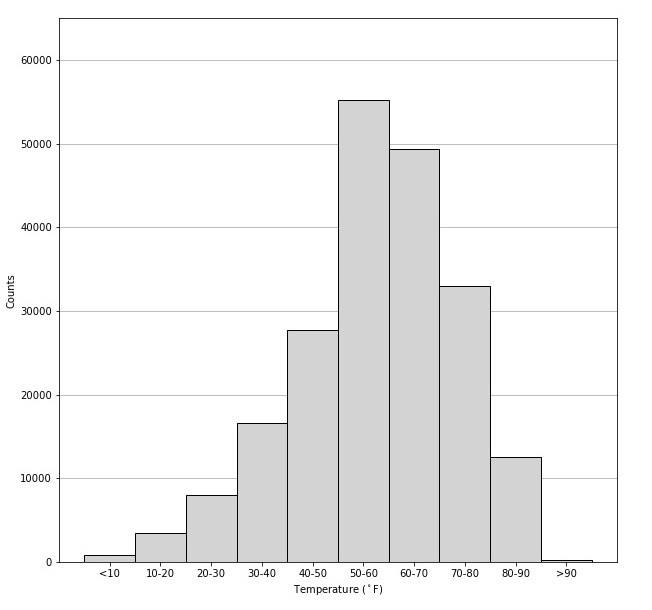
\includegraphics[width=0.9\textwidth]{paper_fig3.jpg}
		
		\label{fig:paper_fig3}
	\end{figure}
	
	\section{Replication of Results}
	\subsection{Statistical Model and Assumptions}
	The authors estimate the following linear probability model: 
	
	$$g_{it} = \beta_0 + \beta_i \text{temp}_{it} + W_{it}\beta_2 + P_{it}\beta_3 + X_{it} \beta_4 + \gamma_i + \Psi_{ct} + \theta_t + \epsilon_{it}$$
	
	$g_{it}$ is a binary variable which indicates whether a judge's decision on application $i$ on date $t$ is granted. temp$_{it}$ is the key variable of interest, which is the average temperature from 6 AM to 4 PM on the date of the court case, with most of the discussion of results centering around $\beta_1$. $W_{it}$ represents a vector of weather controls in the vicinity of the courthouse for application $i$ on date $t$, and $P_{it}$ is a vector for pollution controls with similar indexing. $X_{it}$ is a vector of court and application controls, specifically the category of application and the nationality of the applicant. $\gamma_i$ represents judge fixed effects to account for variation in grant probabilities between judges, and $\Psi_{ct}$ is a vector of city-by-month fixed effects where $c$ indexes over the cities that court-houses are located in, and $t$ represents the month. Lastly, $\theta_t$ includes time fixed effects which controls for day of week and year trends in the data. 
	
	The authors identify the effect off within-location, within-month variation. Their main assumption is that by controlling for location and time effects, the realization of outdoor temperature on a particular given day is as good as random. Since these changes to temperature are basically exogenous, this allows for insight into the effect of temperature on the probability of an affirmative decision.
	
	The authors note that while they have a rich set of fixed effects, there might still be some unobserved characteristics that are important determinants of outcomes that were omitted. However they reason that controlling for location and time fixed effects is plausibly enough to make these omitted characteristics uncorrelated with the case-day temperature, hence the estimates for $\beta_1$ and are unbiased and the associated standard errors remain undisturbed.  
	
	Lastly, they acknowledge that the data could potentially be serially and spatially correlated. As a result, their standard errors are clustered by city-month, which accounts for both of these issues. 
	
	\subsection{Main Results}
	
	We reproduce the authors' results in Table \ref{tab:paper_tab2}. Although using the same datasets as the authors and following the same procedure, albeit using the \verb*|pandas| package in Python for auxiliary data cleaning and the \verb*|felm| package in R to handle the fixed effects linear regression estimation, we end up with a slightly larger number of observations (207,207 in comparison to 206,924). This is an increase of only 283 observations, or an increase of less than 0.1\%. Perhaps as a result of this discrepancy of units, our point estimates are on average around 2\% smaller than those produced by the authors. However, our point estimates all have the same sign, and our standard errors all remain close to the original results. Furthermore, the $F$-statistics all increase for our model results, indicating that there is stronger evidence that the weather variables are jointly significant. As a result of this, our $p$-values for the $F$- tests are also smaller. The authors also run a regression where they include the 3 lag and lead terms and plot the coefficients and confidence intervals, which we reproduce in Figure \ref{fig:paper_fig4}. 
	
	Since our independent variables are divided by 1000, this first converts the unit of our point estimates from proportions to percentages out of 100. The additional factor of 10 then considers a unit change of our independent variable as a change of 10 degrees Fahrenheit. Hence the results imply that a 10 degree increase in daily average temperature from 6AM to 4PM will decrease the probability of an affirmative decision by roughly 1.03\%. Considering that the average affirmative decision baseline is 16.4\%, this implies a 6.55 percent decrease in grant rate. To rephrase this, when the weather is 10 degrees hotter on any given day, the probability of having one's asylum application granted will decrease by 6.55\%. 
	
	
	\begin{table}[h!]
		
		\caption{Main Results}
		\makebox[\textwidth][c]{
			\begin{tabular}{@{\extracolsep{5pt}}lcccc} 
				\\[-1.8ex]\hline 
				\hline \\[-1.8ex] 
				
				& Base & 1 Day Lag & 1 Day Lead & 1 Day Lag/Lead \\ 
				\\[-1.8ex] & (1) & (2) & (3) & (4)\\ 
				\hline \\[-1.8ex] 
				Temperature$_t/1,000$ & $-$1.038$^{***}$ & $-$1.443$^{***}$ & $-$1.187$^{***}$ & $-$1.590$^{***}$ \\ 
				& (0.327) & (0.403) & (0.381) & (0.484) \\ 
				& & & & \\ 
				Temperature$_{t-1}/1,000$ &  & 0.357 &  & 0.367 \\ 
				&  & (0.276) &  & (0.276) \\ 
				& & & & \\ 
				Temperature$_{t+1}/1,000$ &  &  & 0.123 & 0.143 \\ 
				&  &  & (0.259) & (0.259) \\ 
				& & & & \\ 
				\hline \\[-1.8ex] 
				$F$-Statistic for Weather Variables & 3.587 & 3.451 & 3.261 & 3.03 \\ 
				$p$-value & 0.00172 & 0.00128 & 0.00213 & 0.00245 \\ 
				Observations & 207,207 & 207,207 & 207,207 & 207,207 \\ 
				\hline 
				\hline \\[-1.8ex] 
				\textit{Note:}  & \multicolumn{4}{r}{$^{*}$p$<$0.1; $^{**}$p$<$0.05; $^{***}$p$<$0.01} \\ 
		\end{tabular}}
		
		\label{tab:paper_tab2}
	\end{table}
	
	
	\begin{figure}[h!]
		\centering
		\caption{Timing of Exposure: 6AM to 4PM.}
		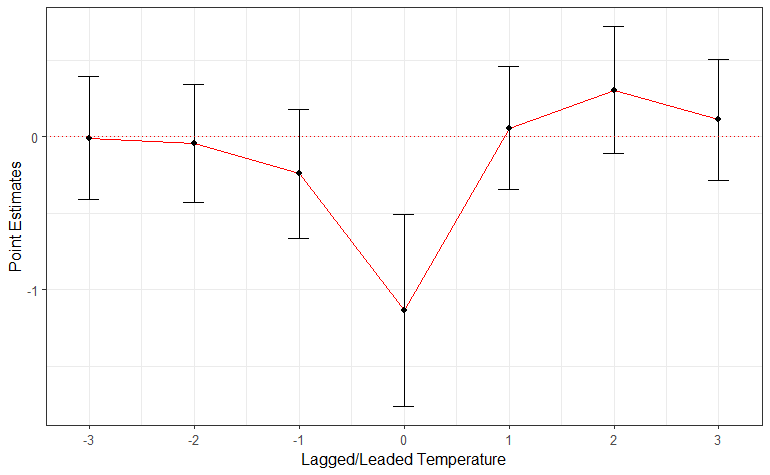
\includegraphics[width=0.7\textwidth]{paper_fig4.jpg}
		\label{fig:paper_fig4}
	\end{figure}
	
	
	
	{\setlength{\tabcolsep}{.4pt}
		\begin{table}[!h] \centering 
			\caption{Alternate Fixed Effects} 
			\label{tab:paper_tab3} 
			\makebox[\textwidth][c]{
				\begin{tabular}{@{\extracolsep{5pt}}lcccccccc} 
					\\[-1.8ex]\hline 
					\hline 
					\\[-1.8ex] & (1) & (2) & (3) & (4) & (5) & (6) & (7) & (8)\\ 
					\hline \\[-1.8ex] 
					Temperature$_t$/1,000 & $-$0.727$^{***}$ & $-$0.737$^{***}$ & $-$0.788$^{***}$ & $-$0.815$^{***}$ & $-$1.031$^{***}$ & $-$0.897$^{***}$ & $-$1.082$^{***}$ & $-$0.933$^{***}$ \\ 
					& (0.269) & (0.272) & (0.269) & (0.248) & (0.277) & (0.214) & (0.269) & (0.283) \\ 
					& & & & & & & & \\ 
					\hline \\[-1.8ex] 
					Nationality FEs & TRUE & TRUE & TRUE & TRUE & TRUE & TRUE & TRUE & TRUE \\ 
					Day of Week FEs & FALSE & TRUE & TRUE & TRUE & TRUE & TRUE & TRUE & FALSE \\ 
					Type of Application FEs & FALSE & FALSE & TRUE & TRUE & TRUE & TRUE & TRUE & TRUE \\ 
					Judge FEs & FALSE & FALSE & FALSE & TRUE & TRUE & TRUE & FALSE & TRUE \\ 
					City-Month FEs & FALSE & FALSE & FALSE & FALSE & TRUE & FALSE & FALSE & TRUE \\ 
					Judge-Month FEs & FALSE & FALSE & FALSE & FALSE & FALSE & FALSE & TRUE & FALSE \\ 
					City FEs & FALSE & FALSE & FALSE & FALSE & FALSE & TRUE & TRUE & FALSE \\ 
					Year FEs & FALSE & FALSE & FALSE & FALSE & FALSE & FALSE & TRUE & TRUE \\ 
					Year-Month FEs & FALSE & FALSE & FALSE & FALSE & FALSE & TRUE & FALSE & FALSE \\ 
					Date FEs & FALSE & FALSE & FALSE & FALSE & FALSE & FALSE & FALSE & TRUE \\ 
					Observations & 207,207 & 207,207 & 207,207 & 207,207 & 207,207 & 207,207 & 207,207 & 207,207 \\ 
					\hline 
					\hline \\[-1.8ex] 
					\textit{Note:}  & \multicolumn{8}{r}{$^{*}$p$<$0.1; $^{**}$p$<$0.05; $^{***}$p$<$0.01} \\ 
			\end{tabular}}
	\end{table}}
	
	The authors believe that their main model includes the most natural set of time fixed effects. However, they also report various permutations of fixed effect variables to examine the stability of their main model. We reproduce these permutations of fixed effects in Table \ref{tab:paper_tab3}, confirming the authors' results that the main selection of fixed effects are valid. 
	
	\subsection{Appraisal of Statistical Assumptions}
	
	The primary point of critique on the author's assumptions is their use of a linear probability model. Binary outcomes and continuous explanatory variables have an inherently nonlinear relationship, as the probability of occurrence is bounded. Hence, although using this model for inference using the current data set gives us estimates of the effect of weather on outcome decisions, it is plausible to believe that out-of-sample analysis might have coefficients that are not accurately represented by the author's results. This linearity is a very strong assumption that the authors are making. However, in the context of advising policy makers, it is the most easily interpreted. Perhaps in the larger picture, the sign, magnitude, and significance are of greater importance than the accuracy of the point estimates. Nonetheless, it could be imagined that this linear probability model does not capture the true causal relationship between temperature and decision outcomes. 
	
	\section{Robustness} 
	
	
	
	{\setlength{\tabcolsep}{.4pt}
		\begin{table}[h!]
			\caption{Robustness Results}
			\begin{tabular}{@{\extracolsep{5pt}}lccccccccc} 
				\\[-1.8ex]\hline 
				\hline 
				\\[-1.8ex] & (1) & (2) & (3) & (4) & (5) & (6) & (7) & (8) & (9)\\ 
				\hline \\[-1.8ex] 
				Temperature & $-$0.907$^{***}$ & $-$1.067$^{**}$ & $-$2.074 & $-$1.567$^{***}$ & $-$1.656$^{***}$ &  &  & $-$0.773$^{*}$ & $-$0.989$^{***}$ \\ 
				& (0.268) & (0.420) & (1.269) & (0.378) & (0.399) &  &  & (0.463) & (0.311) \\ 
				& & & & & & & & & \\ 
				Heat Index &  &  &  &  &  & $-$0.431$^{**}$ & $-$2.007$^{***}$ &  &  \\ 
				&  &  &  &  &  & (0.197) & (0.758) &  &  \\ 
				& & & & & & & & & \\ 
				\hline \\[-1.8ex] 
				Observations & 207,207 & 135,428 & 13,997 & 134,051 & 111,475 & 207,204 & 29,458 & 104,266 & 172,743 \\ 
				\hline 
				\hline \\[-1.8ex] 
				\textit{Note:}  & \multicolumn{9}{r}{$^{*}$p$<$0.1; $^{**}$p$<$0.05; $^{***}$p$<$0.01} 				
			\end{tabular}
			\label{tab:paper_tab5}
			
	\end{table}}
	
	In the following section, we replicate the suite of robustness tests the author conducts. In their paper, they consider a variety of effects that might confound the relationship between temperature and decisions. First, they consider the impact of pollution, and reason that if certain measures of pollution are confounding, then dropping the vector of pollution controls should drastically change the coefficient on temperature in the regression. In column (1) of Table \ref{tab:paper_tab5}, we replicate their results and obtain similar estimates (their coefficient is -0.910, ours is -0.907, a difference of 0.003). Since the magnitude and sign are relatively undisturbed compared to the original point estimate (-1.038), it is likely that pollution is not a large confounder as the coefficients do not change drastically.
	
	Decisions made in California consist of almost 32\% of the observations (roughly 71,000 of the 207,000 decisions). In order to check if there is something different going on in California that is swaying the results of their regression, the authors exclude all decisions made in California and rerun their main specification. We achieve similar results to the authors in column (2) of Table \ref{tab:paper_tab5} (a coefficient of -1.067 compared to -1.159) and conclude that there are no idiosyncrasies associated with California.
	
	Existing research points to how cloud cover could influence mood, hence the authors test running their model on observations where decisions were made on "clear sky" days - the cloud cover was less than 5 percent. Our results are in column (3) of Table \ref{tab:paper_tab5} and we obtained a smaller coefficient than the authors (-2.074 compared to -2.738), however the overall conclusion remains the same. This suggests that there is a more pronounced negative effect of hotter temperatures on clear sky days, however, like the authors, our results are not significant on the 5 percent level. Although the authors make no attempt at explaining this higher result, a possible explanation could be how direct sunlight causes the perceived temperature to be higher than actual ambient levels.
	
	Additionally, the authors explain that research has also pointed to how rain can influence people's moods. The authors then take a subset of data where there was zero precipitation, arguing that these observations cannot have rain influencing the outcomes. Running the regression results in coefficients that retain the sign and significance, however with a larger magnitude and this can be seen in column (4) of Table \ref{tab:paper_tab5}. The authors get a coefficient of -1.304 while we have a slight increase at -1.567. The authors also extend to considering days that had no rain before or after to further solidify that rain could have no effect on these decisions. We replicate this in column (5) of Table \ref{tab:paper_tab5} and have a rather large difference from the authors. Our coefficient ends up being -1.656 while the authors obtain a coefficient of -1.281. Similar to the clear skies results, rain is typically associated with cloudy weather. Hence, this is potentially just a rerun of that regression, with fewer observations. On days with no rain, the lack of clouds might make the temperature be perceived to be hotter, hence resulting in the larger coefficient.  
	
	After considering weather impacts on judge's decision making, the authors consider using a new measure called the Heat Index used by the US National Weather Service which combines both air temperature and relative humidity through a nonlinear algorithm. They posit that this better captures the way that temperature is experienced by humans since different weather conditions can cause the same temperature to be felt hotter or cooler. Simply put, how the weather feels can vary day to day even if the temperature is the same. By re-estimating the results using this heat index instead of just using base temperature, the authors obtain a lower and less significant result when considering all observations, and our replication matches this in column (6) of Table \ref{tab:paper_tab5}. The authors get a coefficient of -0.44 compared to our -0.431. This is in comparison to the original coefficient of -1.038. The overall effect of temperature is cut in half when using a new metric. The authors note that the heat index is typically only considered reliable on warm days, so they then consider only observations where the heat index was greater than 75. We match their results in column (7) of Table \ref{tab:paper_tab5}, obtaining a coefficient that is negative, slightly large in magnitude, and significant (-2.007 for us compared to -1.991). 
	
	Lastly, the authors consider discrepancies in judge's granting rates, as judges do not have specific quotas, and hence some judges are more likely to grant or deny than others. To convince themselves that outlier judges are not driving the results, they drop the first and last quartiles and deciles and reconduct the analysis. We replicated the same results in columns (8) and (9) of Table \ref{tab:paper_tab5} with a coefficient of -0.773 compared to -0.707 for excluding the bottom and top quartiles and a coefficient of -0.989 compared to -1.064 for dropping the top and bottom deciles. Both of these are very close to our original estimate of the effect size at -1.038, and hence outlier judges are likely to not be an issue.
	
	
	\section{Reanalysis} 
	
	In the following section, we attempt to reanalyze the authors' main result first leverage score analysis and then consider a different statistical assumption for the relationship between the covariates and the probability of a favorable decision by running a logit regression for a binary outcome instead of a linear probability model. The use of leverage scores is justified as it allows for us to examine which observations might be potentially driving the results, as outliers may cause the coefficients to be biased. A logit model is justified as the relationship between covariates and approval probability may not be linear as assumed by the authors' model. We instead choose to use a logit model, to see how shifting that assumption might alter the results. We then compute the average marginal effect of temperature on the outcome and compare this with the base result. 
	
	\subsection{Leverage Score Analysis (Observation Level)}
	
	We re-analyze the author's results by first taking a look at the leverage scores of their data from their linear probability model. As seen from Figure \ref{fig:leverage_scores1}, there is a \textit{highly} skewed distribution of leverage scores, with a select subset of the data vastly larger than the majority of the data. In Figure \ref{fig:leverage_scores2}, we only look at the leverage scores less than 0.005. Looking to the right of the figure is the empirical density plot of the leverage scores, and you can see it is no longer as highly skewed as before. Leverage scores indicate the impact each observation has with regards to the overall observation, and give a rough measure of how much the observation influences the fitted value, and hence the coefficients. Hence, we hypothesize that only a select subset is driving the results of the regression, and dropping them will drastically change the coefficients of interest. 
	
	We proceed by dropping high-leverage observations and re-running the base model the authors use with the remaining observations. Since various cutoffs can be used to determine what leverage score is considered to be "too high", we use three decreasing thresholds and examine the impact on the coefficient and confidence interval for temperature. First, we drop all observations with leverage scores greater than 0.05, then with scores greater than 0.01, and lastly with scores greater than 0.0025. Our results are summarized in Table \ref{tab:leverage_reanalysis}. The first column lists the author's results. Our first cutoff at 0.05 removes 1162 observations and causes a \textit{very} slight decrease in the coefficient. At the next cutoff of 0.01, we remove a total of just under 20,000 observations, and there is a further decrease. At the last cutoff of 0.05, we remove almost 50,000 observations, yet still, the results remain the same, albeit with wider confidence intervals due to the fewer observations. Even removing the most influential observations, the author's results remain very stable and still significant, reassuring the validity of their results. 
	
	\begin{figure}[h!]
		\centering
		\caption{Plot of all leverage scores.}
		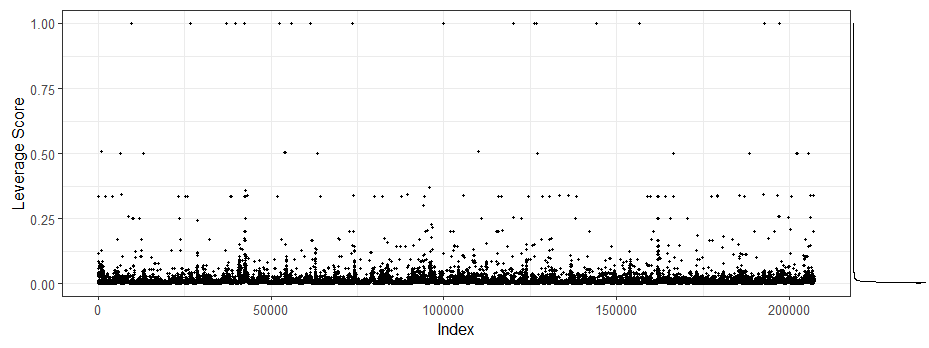
\includegraphics[width=\textwidth]{leverage_scores_1.jpg}
		\label{fig:leverage_scores1}
	\end{figure}
	
	\begin{figure}[h!]
		\centering
		\caption{Plot of leverage scores less than 0.005.}
		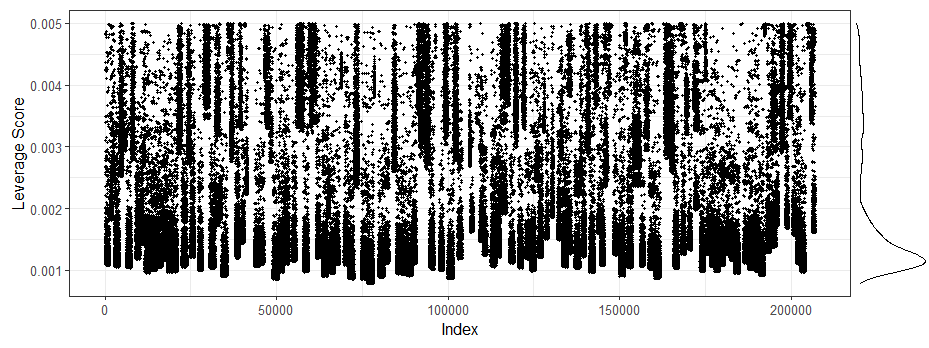
\includegraphics[width=\textwidth]{leverage_scores_4.jpg}
		\label{fig:leverage_scores2}
	\end{figure}
	
	\begin{table}[!h] \centering 
		\caption{Leverage Score Reanalysis} 
		\label{tab:leverage_reanalysis} 
		\begin{tabular}{@{\extracolsep{5pt}}lcccc} 
			\\[-1.8ex]\hline 
			\hline \\[-1.8ex] 
			& $\leq$ 1 & $\leq$ 0.05 & $\leq$0.01 & $\leq$ 0.005 \\ 
			\\[-1.8ex] & (1) & (2) & (3) & (4)\\ 
			\hline \\[-1.8ex] 
			Temperature$_t/1,000$ & $-$1.038$^{***}$ & $-$1.051$^{***}$ & $-$1.147$^{***}$ & $-$1.052$^{**}$ \\ 
			& (0.327) & (0.326) & (0.362) & (0.420) \\ 
			& & & & \\ 
			\hline \\[-1.8ex] 
			F-Statistic for Weather Variables & 3.587 & 3.557 & 3.202 & 3.739 \\ 
			p-value & 0.00172 & 0.00187 & 0.00473 & 0.00164 \\ 
			Observations & 207,207 & 206,045 & 187,903 & 159,706 \\ 
			\hline 
			\hline \\[-1.8ex] 
			\textit{Note:}  & \multicolumn{4}{r}{$^{*}$p$<$0.1; $^{**}$p$<$0.05; $^{***}$p$<$0.01} \\ 
		\end{tabular} 
	\end{table} 
	
	\subsection{Leverage Score Analysis (Cluster Level)}
	
	Looking at Figure \ref{fig:leverage_scores2}, one might notice the vertical groupings of leverage scores between sections in the indexing. The observations are grouped by judges and one can see that some judges have higher or lower minimums for their leverages. This motivated us to consider dropping groups of observations rather than only individual observations that have high leverage. Perhaps an entire group of observations impacts the results rather than one particular observation from a specific judge or a specific city. We plot the average leverage score from grouped data in three different groupings, the identity of a judge, the country of origin for each case, and lastly, the city in which the courthouse is located, which can be seen in Figure \ref{fig:judge_leverages}, \ref{fig:county_leverages}, and \ref{fig:city_leverages}. Using the same process as before, we set a threshold for too large of a leverage score, drop the observations that belong in that subset, and rerun the analysis. Our results are reported in Table \ref{tab:grouped_reanalysis}. Once again, the authors' results are highly stable, and even removing highly influential groups of observations do not greatly affect the coefficient of interest. 
	
	\begin{table}[h] \centering 
		\caption{Grouped Leverage Score Reanalysis} 
		\label{tab:grouped_reanalysis} 
		\begin{tabular}{@{\extracolsep{5pt}}lccc} 
			\\[-1.8ex]\hline 
			\hline \\[-1.8ex] 
			& Judges & Nationality & Courthouse City \\ 
			\\[-1.8ex] & (1) & (2) & (3)\\ 
			\hline \\[-1.8ex] 
			Temperature$_t/1,000$ & $-$1.092$^{***}$ & $-$1.084$^{***}$ & $-$1.109$^{***}$ \\ 
			& (0.335) & (0.325) & (0.338) \\ 
			& & & \\ 
			\hline \\[-1.8ex] 
			F-Statistic for Weather Variables & 3.493 & 3.661 & 3.586 \\ 
			p-value & 0.00217 & 0.00143 & 0.00183 \\ 
			Observations & 202,998 & 205,815 & 202,288 \\ 
			\hline 
			\hline \\[-1.8ex] 
			\textit{Note:}  & \multicolumn{3}{r}{$^{*}$p$<$0.1; $^{**}$p$<$0.05; $^{***}$p$<$0.01} \\ 
		\end{tabular} 
	\end{table} 
	
	
	\begin{figure}[h]
		\centering
		\caption{Mean Leverage Scores grouped by Judge. Cutoff at 0.025}
		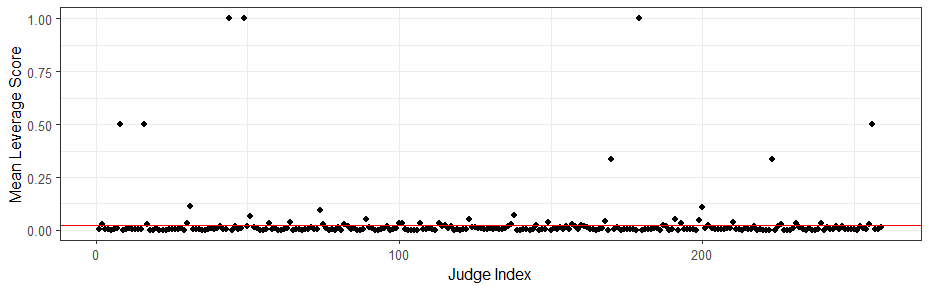
\includegraphics[width=\textwidth]{judge_leverages.jpg}
		\label{fig:judge_leverages}
	\end{figure}
	
	
	\begin{figure}[h]
		\centering
		\caption{Mean Leverage Scores grouped by County of Origin. Cutoff at 0.025}
		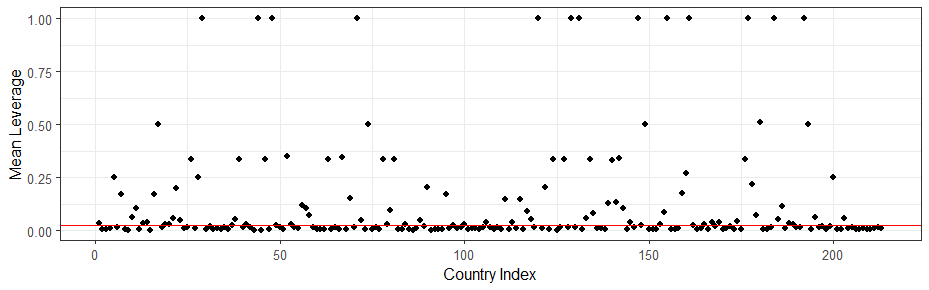
\includegraphics[width=\textwidth]{county_leverages.jpg}
		\label{fig:county_leverages}
	\end{figure}
	
	\begin{figure}[h]
		\centering
		\caption{Mean Leverage Scores grouped by City. Cutoff at 0.045}
		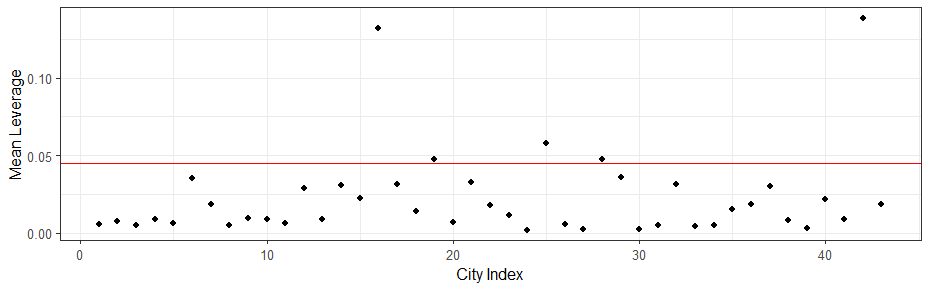
\includegraphics[width=\textwidth]{city_leverages.jpg}
		\label{fig:city_leverages}
	\end{figure}
	
	
	
	\subsection{Logit Model}
	
	We re-analyze the author's assumption of a linear probability model and see whether their results are robust to a different assumption regarding the relationship between covariates and probability. Using a Logit model with the same preferred specification used in the authors' main result, we obtain a coefficient of -9.802 for daily average temperature. A logit model assumes that the relationship between the coefficients and the log-odds of the outcome is linear, hence we must convert this to the average marginal effect of temperature to compare this to the authors' results. After computing this value, we obtain an average marginal effect of -1.0972, with a standard error of 0.2267, which is slightly larger in magnitude and more significant when compared to the authors' result of a point estimate of -1.038 and a standard error of 0.326. However, this is still quite close, indicating that the authors' results are quite robust.
	
	


%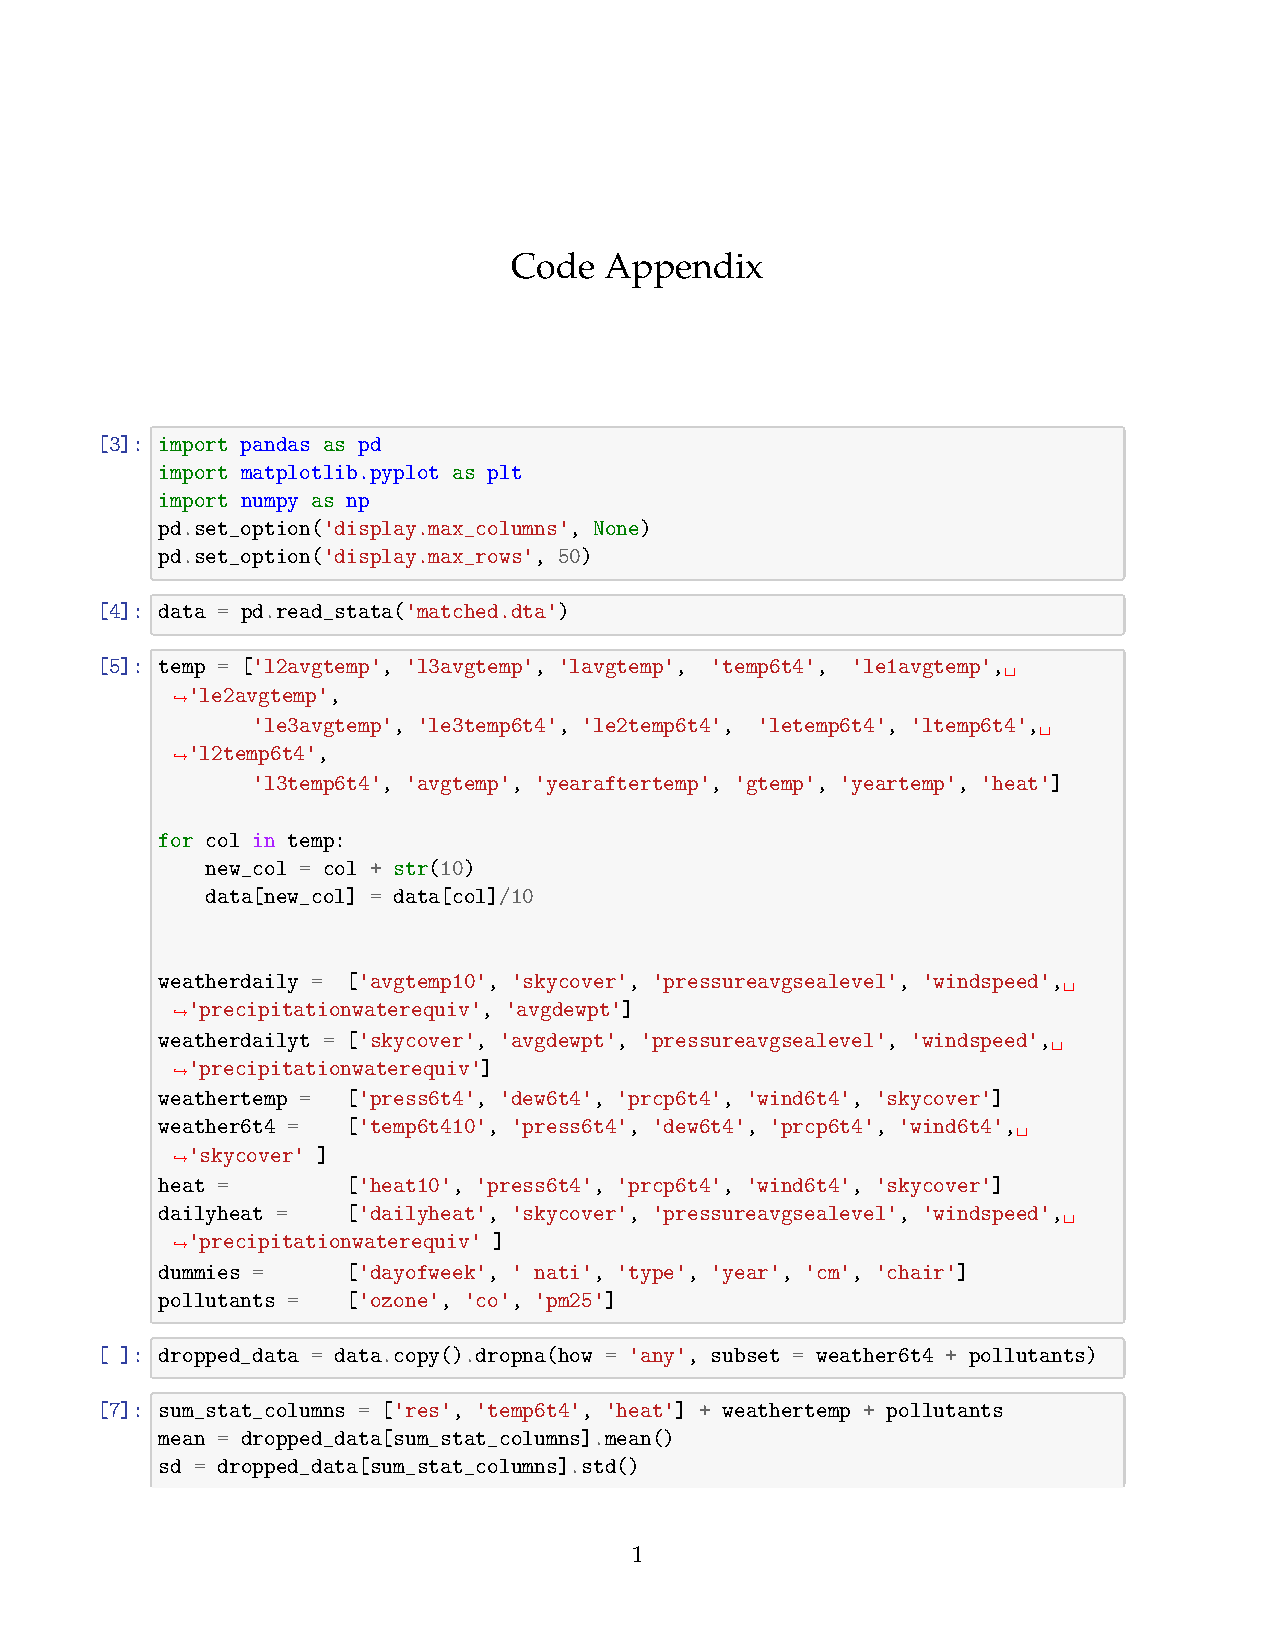
\includepdf[pages=-]{code_appendix.pdf}

%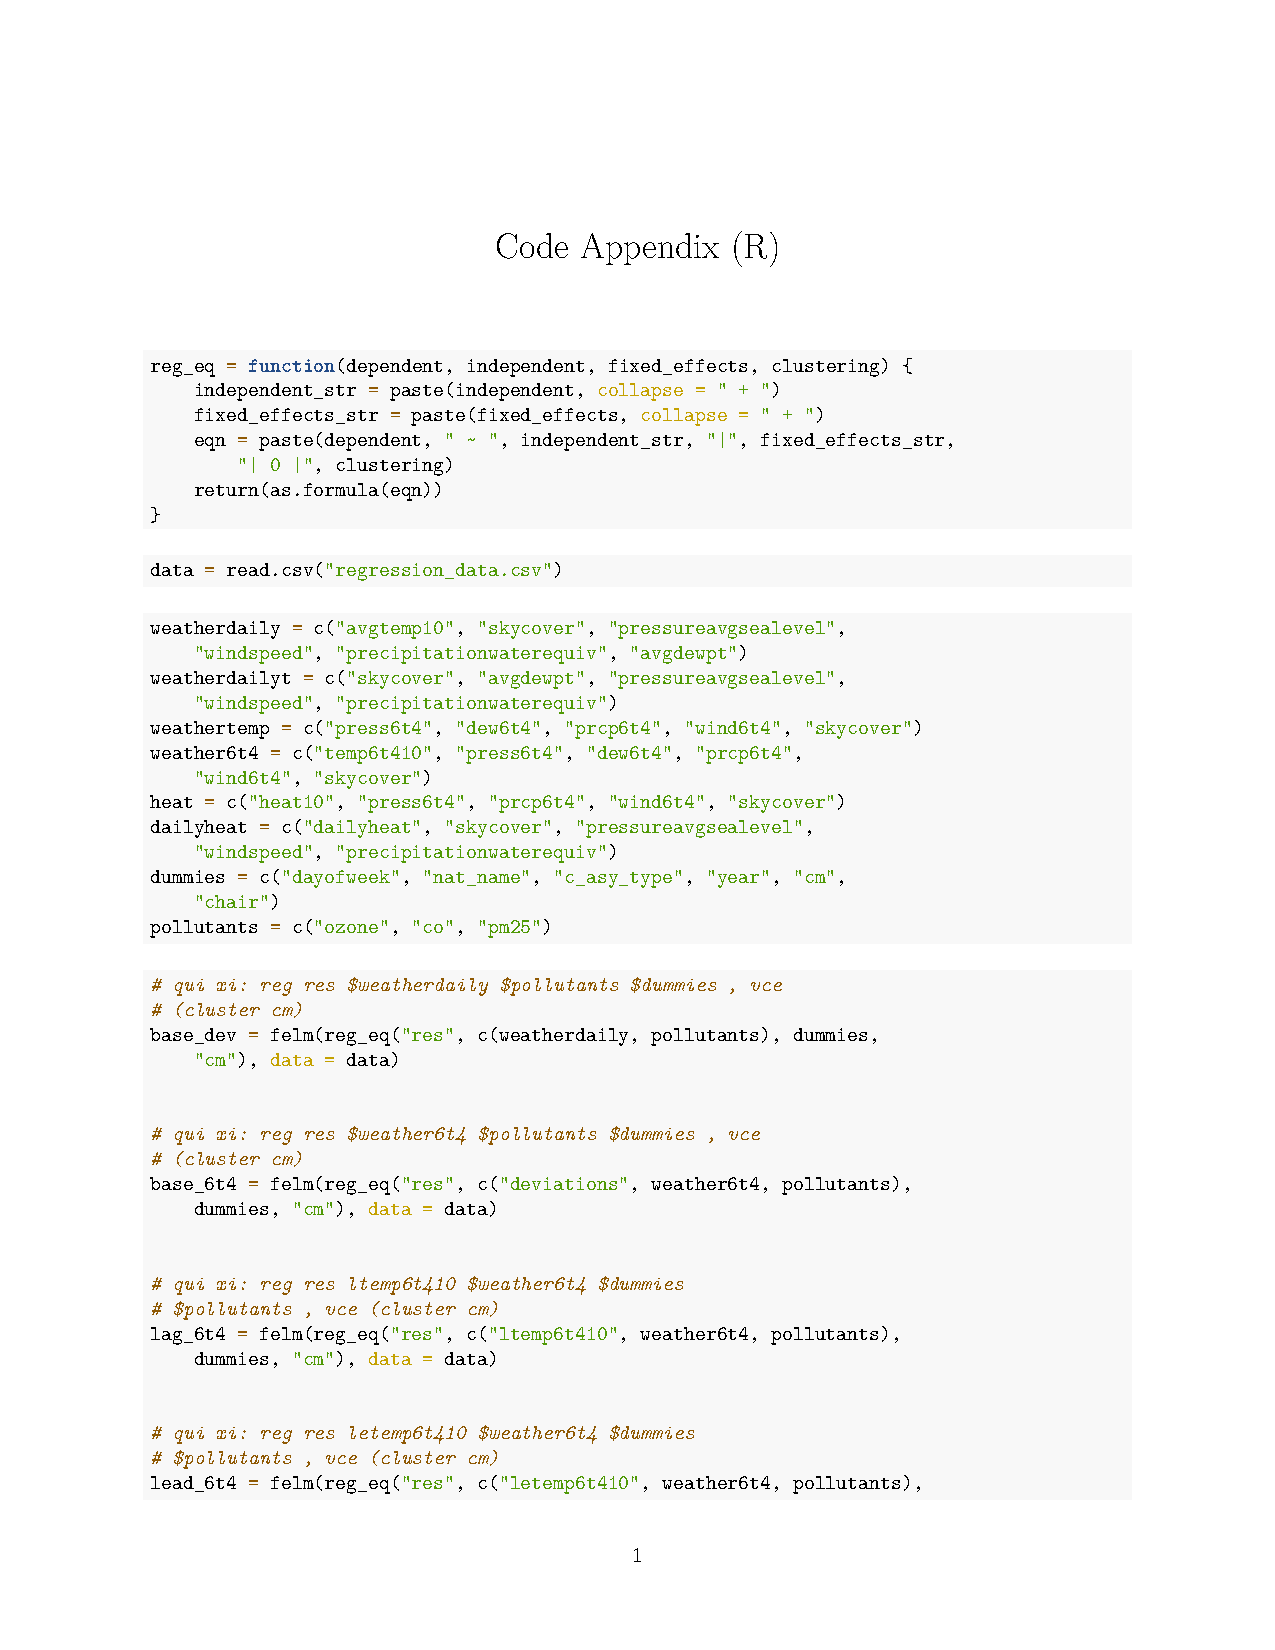
\includepdf[pages=-]{code_appendix_2.pdf}\\


	
\end{document}
